\documentclass{ctexart}

% 导入绘图包
\usepackage{tikz}
% 导入计算点坐标所用的包
\usetikzlibrary{calc}


\begin{document}

\section{线段}

\begin{tabular}{c|c}
    \hline
    带标注的线段
    &\begin{tikzpicture}
        % 设置点的坐标,方便引用
        % 添加点的标注,以及标注的位置
        \coordinate[label=left:\textcolor{blue}{$A$}] 
            (A) at (0, 0);
        \coordinate[label=right:\textcolor{blue}{$B$}] 
            (B) at (1.25, 0.25);

        \draw[red] (A) -- (B);
    \end{tikzpicture}\\
    \hline
    应用随机坐标的线段
    &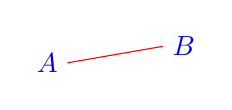
\begin{tikzpicture}
        % 随机坐标(使图形更加自然),rand代表-1到1之间的任意数
        % 方法一可移植性较差,故选用第二种方法(需要导入`calc`包)
        % \coordinate[label=left:\textcolor{blue}{$A$}] 
        %   (A) at (0+0.1*rand, 0+0.1*rand);
        % \coordinate[label=right:\textcolor{blue}{$B$}] 
        %   (B) at (1.25+0.1*rand, 0.25+0.1*rand);
        \coordinate [label=left:\textcolor{blue}{$A$}] 
            (A) at ($(0, 0) + .1*(rand, rand)$);
        \coordinate [label=right:\textcolor{blue}{$B$}] 
            (B) at ($(1.25, 0.25) + .1*(rand, rand)$);
        
        \draw[red] (A) -- (B);
    \end{tikzpicture}\\
    \hline
\end{tabular}

\section{圆与一些交点}

\begin{tabular}{c|c}
    \hline
    一个圆&
    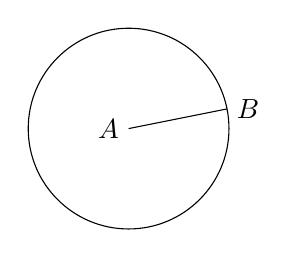
\begin{tikzpicture}
        \coordinate [label=left:$A$] (A) at (0,0); 
        \coordinate [label=right:$B$] (B) at (1.25,0.25); 

        \draw (A) -- (B);
        \draw (A) let \p1 = ($ (B) - (A) $) 
            in circle ({veclen(\x1,\y1)});
    \end{tikzpicture}\\
    \hline
\end{tabular}

\end{document}